% !TeX root = ../../Skript.tex
\cohead{\Large\textbf{Funktionsgleichungen aufstellen}}
\fakesubsection{Funktionsgleichungen aufstellen}
Beim Aufstellen von Funktionsgleichungen vom Typ \(f(x)=a\cdot e^{kx}+b\) können wir in den allermeisten Fällen die folgenden Schritte abarbeiten:
\begin{enumerate}[label=\arabic*)]
	\item Asymptote bestimmen, sofern notwendig. Bei Funktionen vom Typ \(f(x)=a\cdot e^{kx}\) ist die Asymptote \(y=0\) bereits gegeben.
	\item Den Faktor \(a\) bestimmen, indem man den y-Achsenabschnitt einsetzt.
	\item Den Faktor \(k\) mit Hilfe einer weiteren Punktprobe bestimmen.
\end{enumerate}

\medskip

Beispiel: Von einer Funktion \(f(x)=a\cdot e^{kx}+b\) ist bekannt, dass \(f(x)\xrightarrow{\hphantom{\ }x\to-\infty\hphantom{\ }}1\) gilt und dass das Schaubild durch den Ursprung und \(A(2\vert-4)\) verläuft.
\textcolor{loes}{
	\begin{enumerate}[label=\arabic*)]
		\item Aus \(f(x)\xrightarrow{\hphantom{\ }x\to-\infty\hphantom{\ }}1\) folgt, dass die Asymptote \(y=1\) ist und damit \(b=1\).
		\item Da das Schaubild durch den Ursprung verläuft, ist der y-Achsenabschnitt 0:
		\begin{align*}
			f(0)&=0\\
			a\cdot e^0+1&=0\ \vert\ -1\\
			a&=-1
		\end{align*}
		\item Punktprobe mit \(A(2\vert-4)\):
		\begin{align*}
			f(2)&=-4\\
			-1\cdot e^{2k}+1&=-4\ \vert\ -1\\
			-e^{2k}&=-5\ \vert\ \cdot(-1)\\
			e^{2k}&=5\ \vert\ \ln\\
			2k&=\ln\left(5\right)\ \vert\ :2\\
			k&=\frac{1}{2}\ln\left(5\right)
		\end{align*}
		Damit ergibt sich \(f(x)=-e^{\frac{1}{2}\ln\left(5\right)x}+1\)
\end{enumerate}}
\newpage
%%%%%%%%%%%%%%%%%%%%%%%%%%%%%%%%%%%%%%%%%%%%%%%%%%%%%%%%%%%%%%%%%%%%%%%%%%%%%%%%%%%%%%%%%%%%%%%%%%%%%%
\begin{Exercise}[title={\raggedright Stelle jeweils eine Funktionsgleichung vom passenden Typ auf}, label=eFktFGlAA1]

    \begin{minipage}{\textwidth}
		\adjustbox{valign=t}{\begin{minipage}{0.5\textwidth}
			\begin{enumerate}[label=\alph*)]
				\item Das Schaubild von \(f_1(x)=ae^{kx}\) verläuft durch die Punkte \(A(0\vert3)\) und \(B(2\vert8)\).
				\item Das Schaubild von \(f_2(x)=ae^{kx}\) verläuft durch die Punkte \(A(0\vert-1)\) und \(B(-2\vert-5)\).
				\item Das Schaubild von \(f_3(x)=ae^{kx}\) verläuft durch die Punkte \(A(0\vert5)\) und \(B(3\vert4)\).
				\item Das Schaubild von \(f_4(x)=ae^{kx}+b\) verläuft durch die Punkte \(A(0\vert5)\) und \(B(-1\vert3)\) und hat die Asymptote \(y=7\).
				\item Das Schaubild von \(f_5(x)=ae^{kx}+b\) verläuft durch die Punkte \(A(0\vert0)\) und \(B(3\vert-3)\) und hat die Asymptote \(y=3\).
				\item Das Schaubild von \(f_6(x)=ae^{kx}+b\) verläuft durch die Punkte \(A(4\vert-2)\) und \(B(0\vert3)\) und hat die Asymptote \(y=-4\).
				\item Von der Funktion \(f_7(x)=ae^{kx}+b\) ist das Verhalten bekannt: \(f_7(x)\xrightarrow{\hphantom{\ }x\to-\infty\hphantom{\ }}-1\) Zudem ist folgende Wertetabelle gegeben:

				\begin{tabular}{c|cc}
					\(x\)&-5&0\\
					\hline
					\(f_7(x)\)&2&8
				\end{tabular}
				\item Von der Funktion \(f_8(x)=ae^{kx}+b\) ist das Verhalten bekannt: \(f_8(x)\xrightarrow{\hphantom{\ }x\to-\infty\hphantom{\ }}2\) Zudem ist folgende Wertetabelle gegeben:

				\begin{tabular}{c|cc}
					\(x\)&-5&0\\
					\hline
					\(f_8(x)\)&0&1
				\end{tabular}
				\item Von der Funktion \(f_9(x)=ae^{kx}+b\) ist das Verhalten bekannt: \(f_9(x)\xrightarrow{\hphantom{\ }x\to-\infty\hphantom{\ }}-4\) Zudem ist folgende Wertetabelle gegeben:

				\begin{tabular}{c|cc}
					\(x\)&0&1\\
					\hline
					\(f_9(x)\)&-3&-1
				\end{tabular}
			\end{enumerate}
		\end{minipage}}%
		\adjustbox{valign=t}{\begin{minipage}{0.5\textwidth}
			\begin{enumerate}[label=\alph*)]
				\setcounter{enumi}{9}
				\item Gegeben ist folgendes Schaubild:

				\begin{minipage}{\textwidth-5.75ex}
					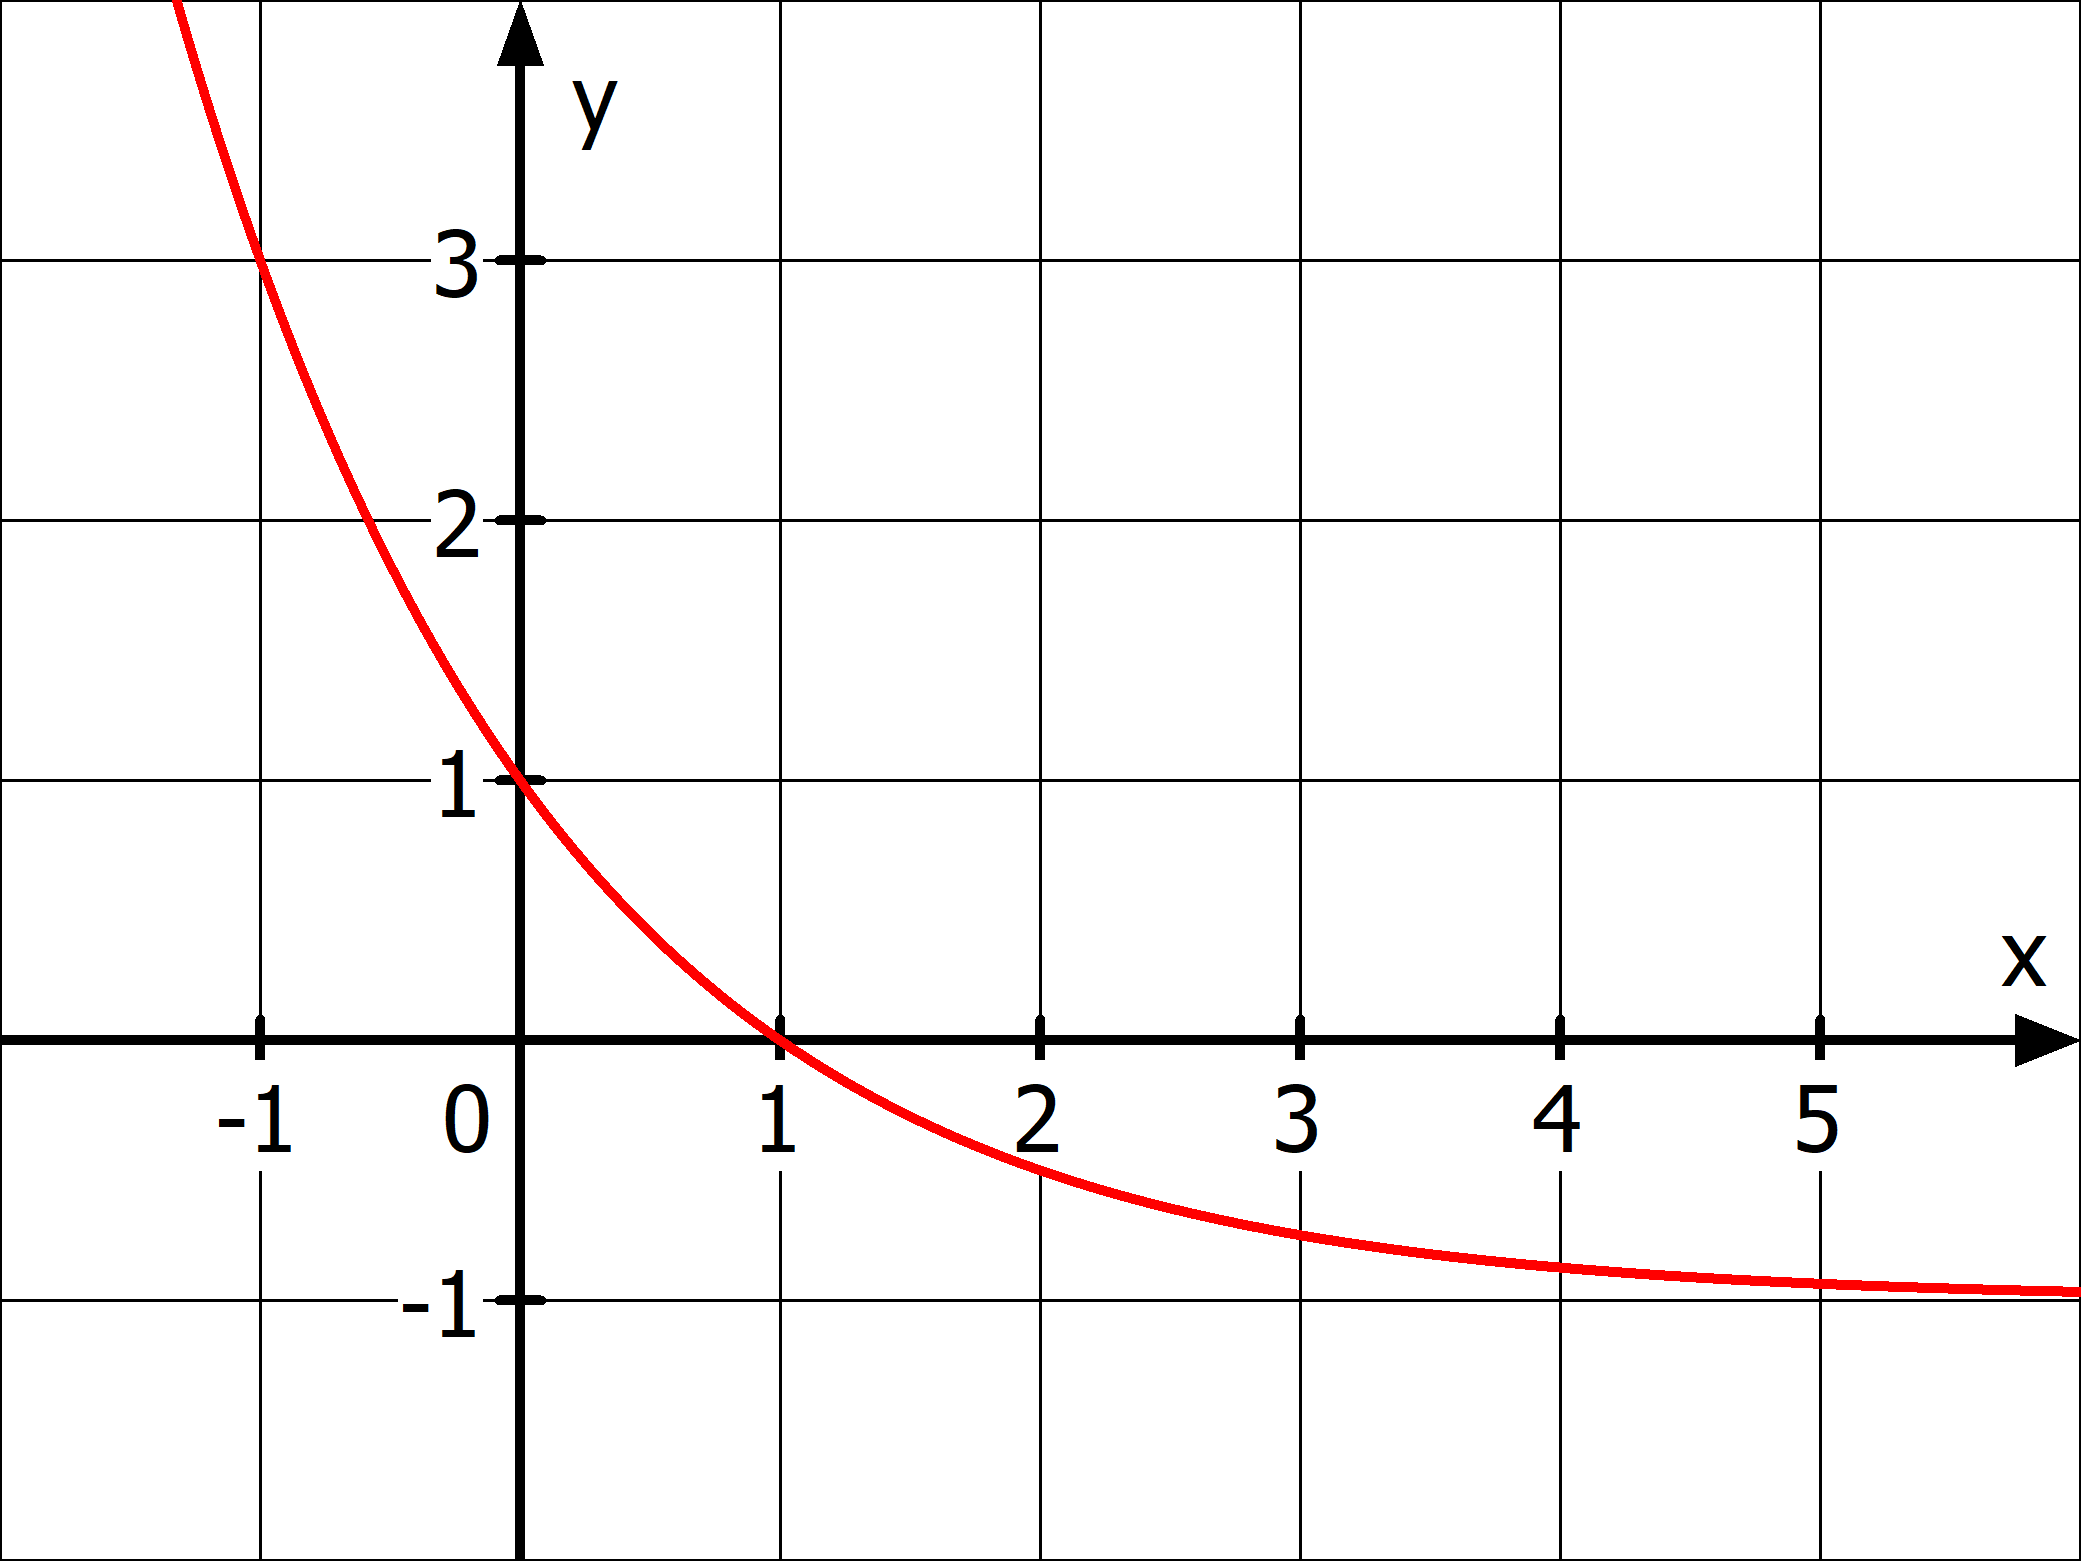
\includegraphics[width=\textwidth]{\eFkt/pics/FktGlAA1.png}
				\end{minipage}%

                \medskip

				\item Gegeben ist folgendes Schaubild:

				\begin{minipage}{\textwidth-5.75ex}
					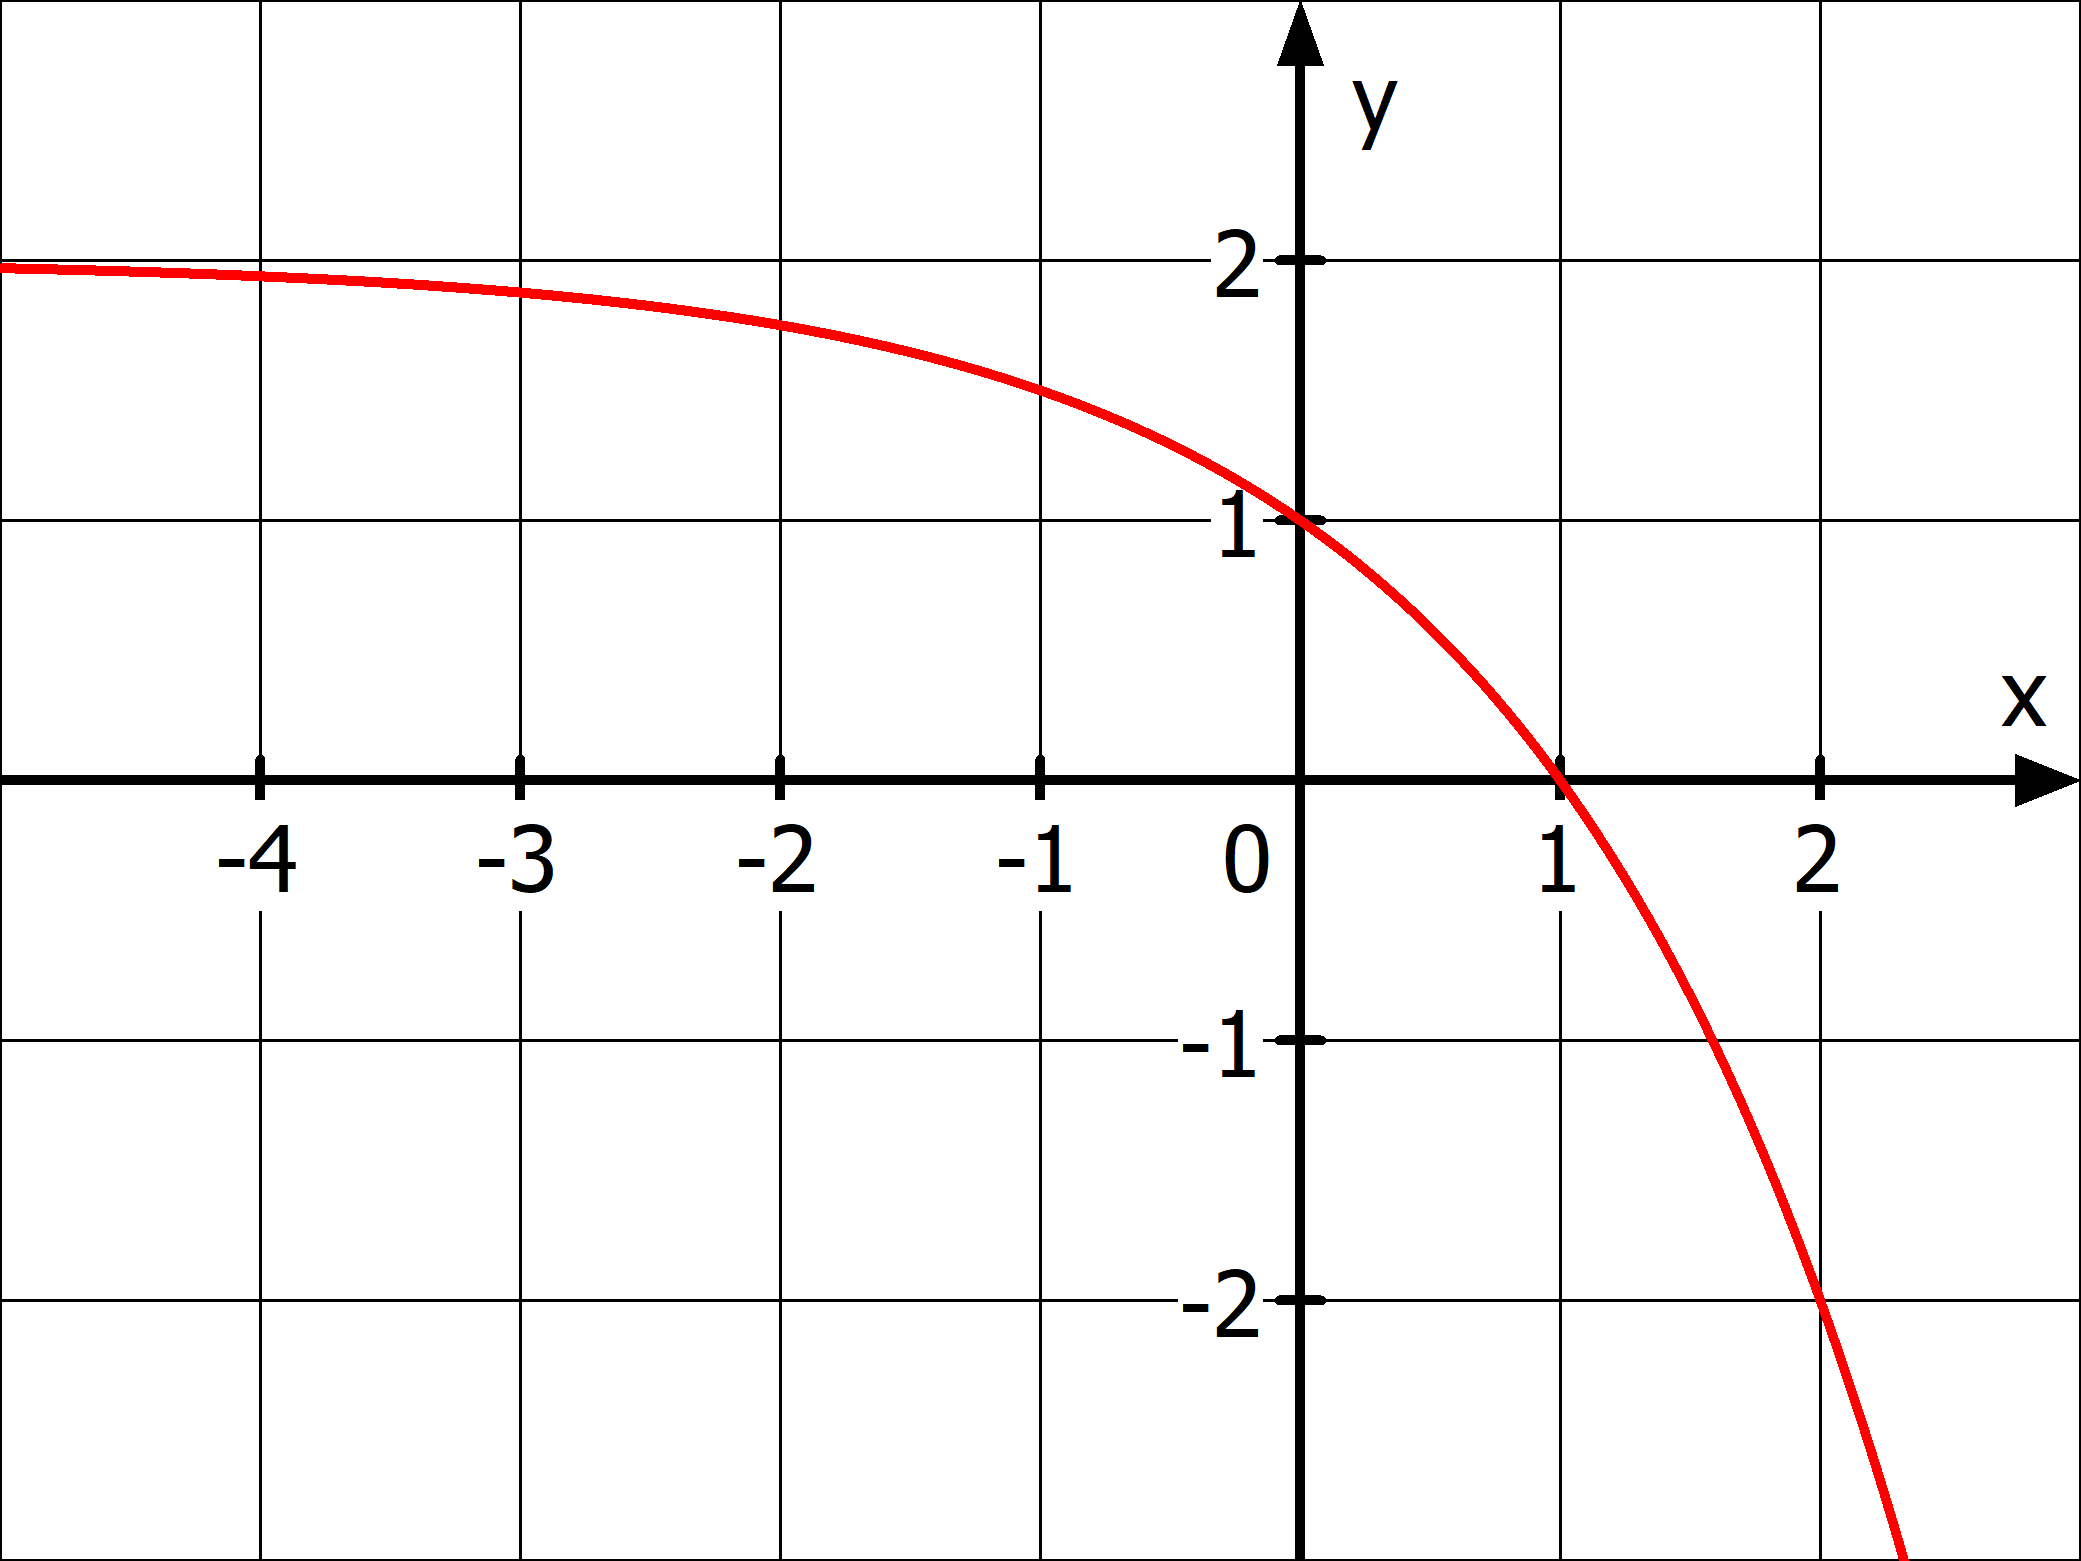
\includegraphics[width=\textwidth]{\eFkt/pics/FktGlAA2.png}
				\end{minipage}%

                \medskip

				\item Gegeben ist folgendes Schaubild:

				\begin{minipage}{\textwidth-5.75ex}
					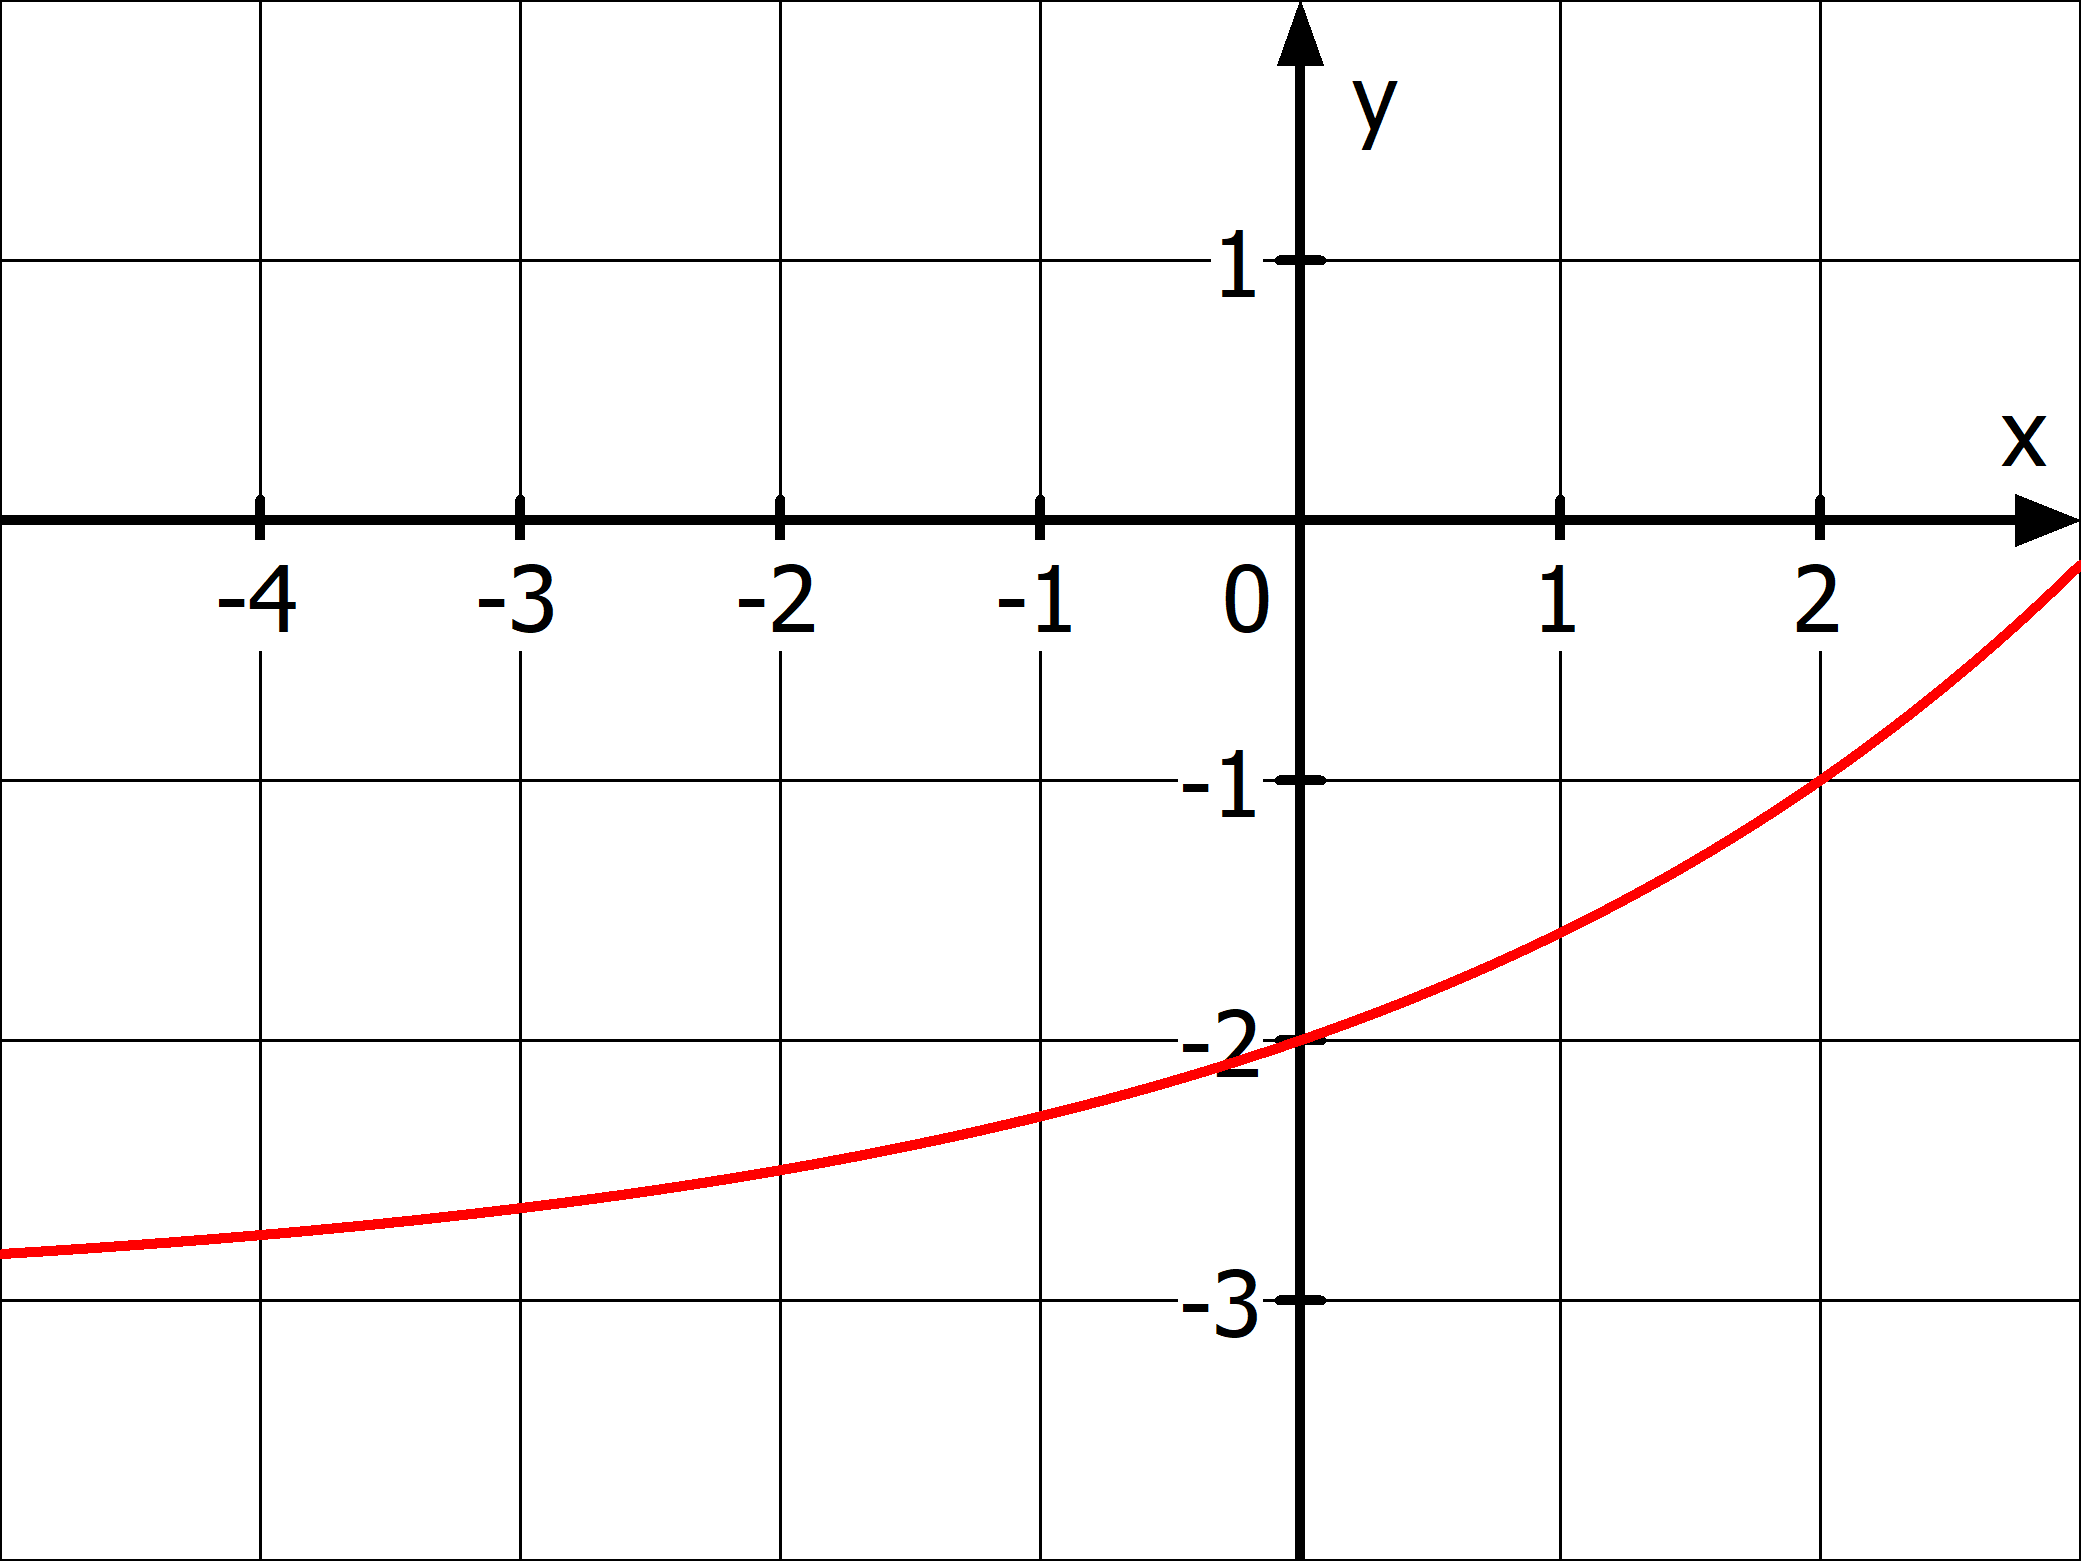
\includegraphics[width=\textwidth]{\eFkt/pics/FktGlAA3.png}
				\end{minipage}%
			\end{enumerate}
		\end{minipage}}%
    \end{minipage}
\end{Exercise}
\newpage
%%%%%%%%%%%%%%%%%%%%%%%%%%%%%%%%%%%%%%%%%
\begin{Answer}[ref=eFktFGlAA1]

	\begin{minipage}{\textwidth}
		\begin{minipage}[t]{0.5\textwidth}
			\begin{enumerate}[label=\alph*)]
				\item \(f_1(x)=3e^{\frac{1}{2}\ln\left(\frac{8}{3}\right)x}\)
				\item \(f_2(x)=-e^{-\frac{1}{2}\ln\left(5\right)x}\)
				\item \(f_3(x)=5e^{\frac{1}{3}\ln\left(\frac{4}{5}\right)x}\)
				\item \(f_4(x)=-2e^{-\ln(2)x}+7\)
				\item \(f_5(x)=-3e^{\frac{1}{3}\ln\left(2\right)x}+3\)
				\item \(f_6(x)=7e^{\frac{1}{4}\ln\left(\frac{2}{7}\right)x}-4\)
			\end{enumerate}
		\end{minipage}%
		\begin{minipage}[t]{0.5\textwidth}
			\begin{enumerate}[label=\alph*)]
				\setcounter{enumi}{6}
				\item \(f_7(x)=9e^{-\frac{1}{5}\ln\left(\frac{1}{3}\right)x}-1\)
				\item \(f_8(x)=-e^{-\frac{1}{5}\ln\left(2\right)x}+2\)
				\item \(f_9(x)=e^{\ln(5)x}-4\)
				\item \(f_{10}(x)=2e^{-\ln(2)x}-1\)
				\item \(f_{11}(x)=-e^{-\ln\left(\frac{1}{2}\right)x}+2\)
				\item \(f_{12}(x)=e^{0,5\ln(2)x}-3\)
			\end{enumerate}
		\end{minipage}%
	\end{minipage}
\end{Answer}